\documentclass[10pt,A4]{article}

% --- isi dari mycv.sty dimasukkan di sini ---

\RequirePackage[utf8]{inputenc}		
\RequirePackage{xifthen}
\RequirePackage[default]{raleway}
\renewcommand*\familydefault{\sfdefault} 		
\RequirePackage[T1]{fontenc}
\RequirePackage{moresize}		
\RequirePackage[a4paper]{geometry}		
\geometry{top=1.75cm, bottom=-.6cm, left=1.5cm, right=1.5cm} 	
\RequirePackage{fancyhdr}				
\setlength{\headheight}{-5pt}		
\lhead{}
\chead{\small{Jan Küster  $\cdot$ Consultant and Software Engineer $\cdot$  Bremen, Germany  $\cdot$  \textcolor{sectcol}{\textbf{info@jankuester.com}}  $\cdot$ +49 176 *** *** **}}
\rhead{}
\setlength{\parindent}{0mm}

\RequirePackage{multicol}			
\RequirePackage{multirow}
\RequirePackage{array}
\newcolumntype{x}[1]{>{\raggedleft\hspace{0pt}}p{#1}}%

\RequirePackage{graphicx}
\RequirePackage{wrapfig}
\RequirePackage{float}
\RequirePackage{tikz}				
\usetikzlibrary{shapes, backgrounds,mindmap, trees}

\RequirePackage{color}
\definecolor{sectcol}{RGB}{255,150,0}
\definecolor{bgcol}{RGB}{110,110,110}
\definecolor{softcol}{RGB}{225,225,225}

\renewcommand{\headrulewidth}{0pt} 
\renewcommand{\footrulewidth}{0pt}	  	
\renewcommand{\thepage}{}	
\renewcommand{\thesection}{}			

% semua custom commands (larrow, cvsection, cvevent, dll)

\newcommand{\tzlarrow}{(0,0) -- (0.2,0) -- (0.3,0.2) -- (0.2,0.4) -- (0,0.4) -- (0.1,0.2) -- cycle;}	
\newcommand{\larrow}[1]{\begin{tikzpicture}[scale=0.58]
	 \filldraw[fill=#1!100,draw=#1!100!black]  \tzlarrow
 \end{tikzpicture}
}
\newcommand{\tzrarrow}{ (0,0.2) -- (0.1,0) -- (0.3,0) -- (0.2,0.2) -- (0.3,0.4) -- (0.1,0.4) -- cycle;}
\newcommand{\rarrow}{
\begin{tikzpicture}[scale=0.7]
	\filldraw[fill=sectcol!100,draw=sectcol!100!black] \tzrarrow
 \end{tikzpicture}
}

\newcommand{\cvsection}[1]
{
\colorbox{sectcol}{\mystrut \makebox[1\linewidth][l]{
\larrow{bgcol}	\hspace{-8pt} \larrow{bgcol} \hspace{-8pt} \larrow{bgcol} \textcolor{white}{\textbf{#1}}\hspace{4pt}
}}\\
}
\newcommand{\metasection}[2]
{
\begin{tabular*}{1\textwidth}{p{2.4cm} p{11cm}}
\larrow{bgcol}	\normalsize{\textcolor{sectcol}{#1}}&#2\\[12pt]
\end{tabular*}
}
\newcommand{\cvevent}[5]
{
\vspace{8pt}
	\begin{tabular*}{1\textwidth}{p{2.3cm}  p{10.8cm} x{3.9cm}}
 \textcolor{bgcol}{#1}& \textbf{#2} & \vspace{2.5pt}\textcolor{sectcol}{#3}
	\end{tabular*}
\vspace{-12pt}
\textcolor{softcol}{\hrule}
\vspace{6pt}
	\begin{tabular*}{1\textwidth}{p{2.3cm} p{14.4cm}}
&		 \larrow{bgcol}  #4\\[3pt]
&		 \larrow{bgcol}  #5\\[6pt]
	\end{tabular*}
}
\newcommand{\cveventmeta}[2]
{
	\mbox{\mystrut \hspace{87pt}\textit{#1}}\\
	#2
}
\newcommand{\mystrut}{\rule[-.3\baselineskip]{0pt}{\baselineskip}}
\newcommand{\lorem}{Lorem ipsum dolor sit amet, consectetur adipiscing elit. Donec a diam lectus.}

% --- selesai isi mycv.sty ---

\begin{document}

\pagestyle{fancy}

\vspace{-20.55pt}
\hspace{-0.25\linewidth}\colorbox{bgcol}{\makebox[1.5\linewidth][c]{\HUGE{\textcolor{white}{\textsc{Jan Küster}} } \textcolor{sectcol}{\rule[-1mm]{1mm}{0.9cm}} \HUGE{\textcolor{white}{\textsc{Resume}} } }}

\begin{figure}[H]
\begin{flushright}
	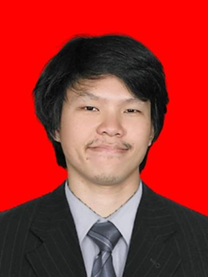
\includegraphics[trim=320 130 460 210,clip,width=0.2\linewidth]{./myfoto.png}
\end{flushright}
\end{figure}

\vspace{-114pt}
\metasection{Status:}{M.Sc. Digital Media, Fullstack JS Engineer}
\metasection{Fields:}{Project Management, Software Development, Consulting} 
\metasection{Tech:}{Meteor, Javascript, Bootstrap, Mongodb, Git, Webstorm, Sourcetree}
\metasection{Loves:}{Global Game Jam, Sci-Fi series, Stackoverflow, Fitness and Martial Arts}

\vspace{6pt}

\cvsection{Experience}
\cvevent{2016 / 09}{Fullstack Javascript Engineer}{University of Bremen}{Invent a realtime classroom management using Meteor and React}{Design software architecture and leading development}
\cvevent{2014 - 2016}{IT Consultant for IBM XPages and Notes Domino}{We4IT GmbH Bremen}{Realize projects in XPages and We4IT Aveedo, monitor project status, conduct reports}{Integrated Camunda BPMN engine and BPMN.IO modeler in We4IT Aveedo}
\cvevent{2012 - 2014}{Scientific Employee / Software Development}{University of Bremen}{Invented a flexible assessment framework, targeting industrial trainees}{Supervised software development lifecycle, Recruited team members}
\cvevent{2011 / 11}{Project Management Simulation Training}{Getoq Consulting}{Performed a two-day project simulation from management perspective}{Topics included customer contracts, change management, controlling, operational tasks}
\cvevent{2010 - 2011}{Student Assistant / Programmer}{otulea.uni-bremen.de}{Realized an online diagnosis platform for workforce literacy development (Flex)}{Modeled software design, implemented various prototypes, conducted usability tests}

\cvsection{Education}
\cvevent{2015 / 07}{Graduated as M.Sc. Digital Media}{University of Bremen}{Master Thesis: Semi Automated Scoring in Technology Based Assessment}{Developed and evaluated an algorithm for semi automated scoring of spreadsheet data}
\cvevent{2012 - 2013}{Master Project - PrIMA}{University of Bremen}{Co-Invented a touch table application for medical support, co-developed software (Java)}{Formed a scrum team, mainted project dev server (Debian), surveyed target audience}
\cvevent{2012 - 2015}{Master Studies Digital Media}{University of Bremen}{Inter-cultural classes in English, covering special topics in computer science and design}{Professionalized in research methods, software development and e-assessment}
\cvevent{2009 - 2010}{Semester Abroad}{University of Melbourne}{Mastered six months of study and trans-cultural experience in Melbourne, Australia}{Finished machine programming, information visualization, professional essay writing}

\null
\vspace*{\fill}
\hspace{-0.25\linewidth}\colorbox{bgcol}{\makebox[1.5\linewidth][c]{\mystrut \small \textcolor{white}{www.jankuester.com} $\cdot$ \textcolor{white}{github.com/jankapunkt}}}

\end{document}
